\documentclass{article}
\usepackage{graphicx}
\usepackage{hyperref}
\usepackage{biblatex}
\addbibresource{sources.bib}

\author{Meftah, Morteza M.D,; Waren, Daniel M.D; Bosco, Joseph A. IV;\\
Di Gangi, Catherine; Watson, Cody Ph.D}
\title{Modeling Robotic Surgery Predictions: Write-Up}

\begin{document}

\maketitle

\textbf{%
This is a VERY rough draft of the write-up. 
It is meant to demonstrate the work I have done on the project in a way that you don't need to read any code.
Document written by Jack Bosco. 
Code for the data analysis, modeling, and visualization are also written by Jack Bosco. 
}

\section{Methods}

\subsection{Data Collection}

The data was collected from a robotic surgery system that was used to perform total knee arthroplasty (TKA) on 100 patients.


\newpage

\begin{figure}[t]
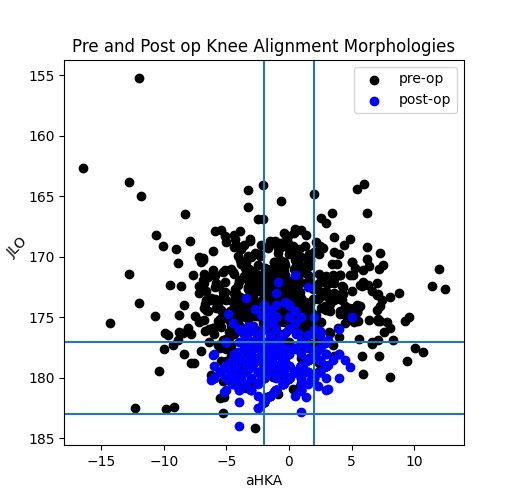
\includegraphics[width=.9\textwidth]{data_vis.png}
\caption{These are the averages of the clusters - See CPAK reference}
\end{figure}

Top: Pre and post-op data displayed on a scatterchart of Joint Line Obliquity (JLO) and anterior Hip Knee Alignment (aHKA)\\
Bottom: Average Pre and post-op alignment grouped by pre-operative aHKA values.
The average change from pre-op to post-op is shown.

\newpage

\begin{figure}[t]
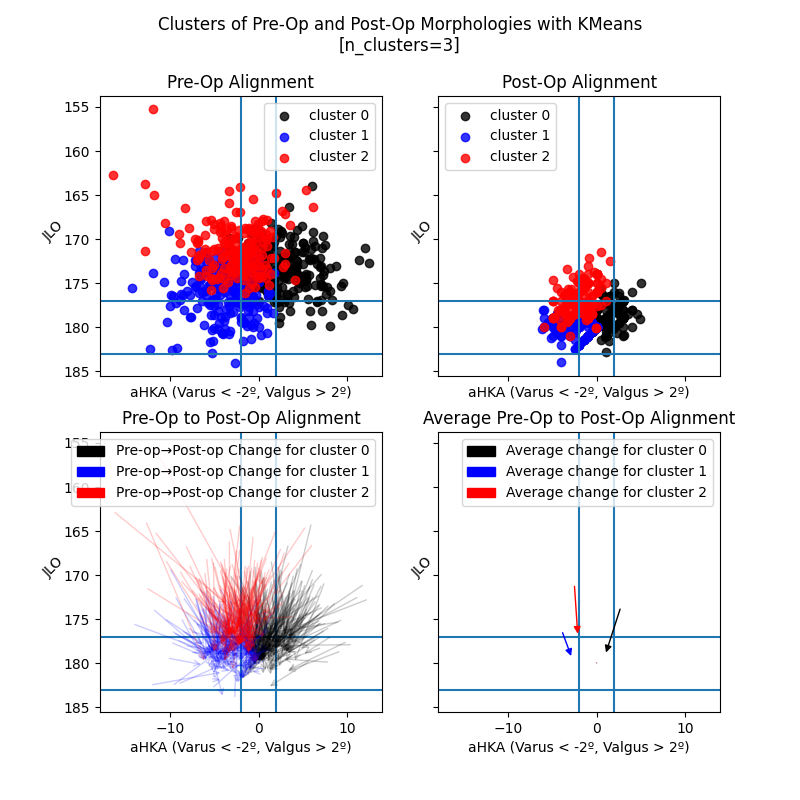
\includegraphics[width=\textwidth]{clusters.png}
\caption{These are the clusered data points.}
\end{figure}

First, the pre-operative data was standardized using the standard scaler method.
Then, the pre-operative alignments were clustered using the K-means clustering algorithm
(see \href{https://scikit-learn.org/stable/modules/generated/sklearn.cluster.KMeans.html#sklearn.cluster.KMeans}
{\underline{Sklearn K-Means Clustering}}).\\
Bottom Left: Arrows are drawn for each pre and post-operative pair (one pair per case).\\
Bottom Right: Averages are taken for each cluser and the change from pre-op to post-op is shown.

\newpage

\begin{figure}[t]
	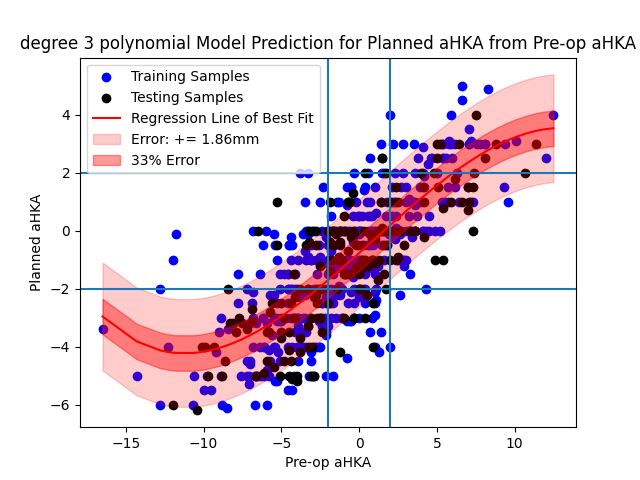
\includegraphics[width=\textwidth]{degree_3_polynomial_regression.png}
	\caption{This is a regression trained using a linear regression algorithm.
	The error is the mean squared distance from the testing set (black). 
	The regression is trained on the training set (blue)}
\end{figure}

To create this regression, the pre and post-operative aHKA values were standardized using the standard scaler method.\\
Then, the features are transformed using a polynomial transformation of degree 3 
(see \href{https://scikit-learn.org/stable/modules/generated/sklearn.linear_model.LinearRegression.html}{\underline{Sklearn Polynomial Features}}).\\
Finally, the model is trained using a linear regression algorithm 
(see \href{https://scikit-learn.org/stable/modules/generated/sklearn.linear_model.LinearRegression.html}{\underline{Sklearn Linear Regression}}).

\newpage

\begin{figure}[t]
	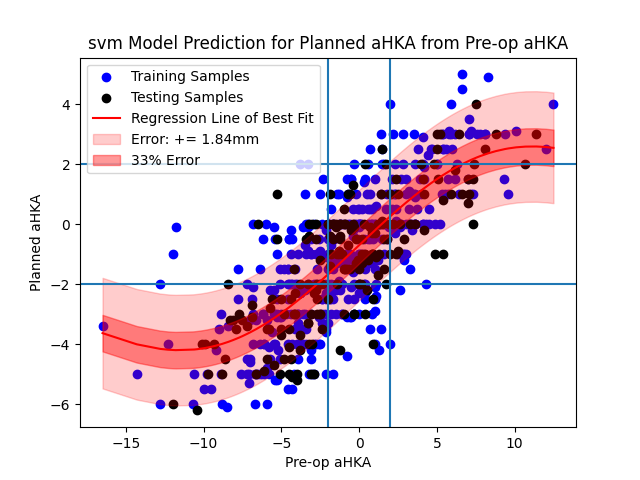
\includegraphics[width=\textwidth]{svm_regression.png}
	\caption{This is a regression trained using a support vector machine algorithm.
	The error is the mean squared distance from the testing set (black). 
	The regression is trained on the training set (blue)}
\end{figure}

To create this regression, the pre and post-operative aHKA values were standardized using the standard scaler method.\\
Then, the model is trained using a nu support vector regression algorithm
(see \href{https://scikit-learn.org/stable/modules/generated/sklearn.svm.NuSVR.html#sklearn.svm.NuSVR}{\underline{Sklearn Support Vector Machine}}).

\newpage

\begin{figure}[t]
	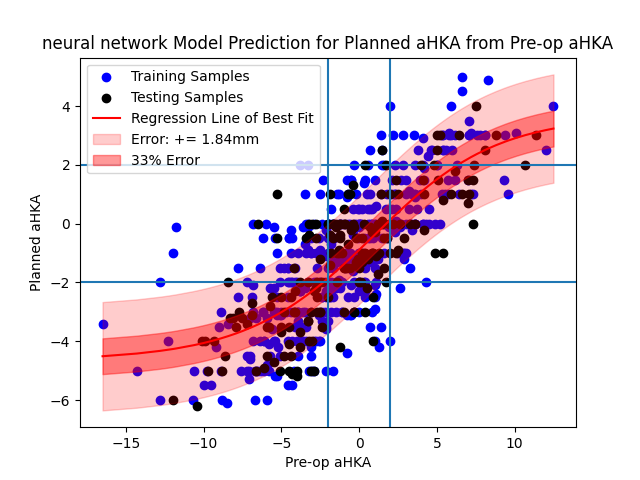
\includegraphics[width=\textwidth]{neural_network_regression.png}
	\caption{This is a regression trained using a deep learning algorithm on a MLP/neural network model.
	The error is the mean squared distance from the testing set (black). 
	The regression is trained on the training set (blue)}
\end{figure}

To create this regression, the pre and post-operative aHKA values were normalized using the min-max scaler
method with feature range $(-1, 1)$.\\
Then, the model is trained using a multi-layer perceptron (MLP) algorithm 
(see \href{https://scikit-learn.org/stable/modules/generated/sklearn.neural_network.MLPRegressor.html}{\underline{Sklearn Multi-layer Perceptrion}}).

\medskip

\printbibliography

\end{document}

